\documentclass[a4paper,12pt]{article}
\usepackage{amsmath,amssymb,amsfonts,amsthm}
\usepackage{tikz}
\usepackage [utf8x] {inputenc}
\usepackage [T2A] {fontenc} 
\usepackage[russian]{babel}
\usepackage{cmap} 
\usepackage{ gensymb }
% Так ссылки в PDF будут активны
\usepackage[unicode]{hyperref}
\usepackage{ textcomp }
\usepackage{indentfirst}
\usepackage[version=3]{mhchem}

% вы сможете вставлять картинки командой \includegraphics[width=0.7\textwidth]{ИМЯ ФАЙЛА}
% получается подключать, как минимум, файлы .pdf, .jpg, .png.
\usepackage{graphicx}
% Если вы хотите явно указать поля:
\usepackage[margin=1in]{geometry}
% Или если вы хотите задать поля менее явно (чем больше DIV, тем больше места под текст):
% \usepackage[DIV=10]{typearea}

\usepackage{fancyhdr}

\newcommand{\bbR}{\mathbb R}%теперь вместо длинной команды \mathbb R (множество вещественных чисел) можно писать короткую запись \bbR. Вместо \bbR вы можете вписать любую строчку букв, которая начинается с '\'.
\newcommand{\eps}{\varepsilon}
\newcommand{\bbN}{\mathbb N}
\newcommand{\dif}{\mathrm{d}}

\newtheorem{Def}{Определение}


\pagestyle{fancy}
\makeatletter % сделать "@" "буквой", а не "спецсимволом" - можно использовать "служебные" команды, содержащие @ в названии
\fancyhead[L]{\footnotesize Квантовая физика}%Это будет написано вверху страницы слева
\fancyhead[R]{\footnotesize ФМХФ МФТИ}
\fancyfoot[L]{\footnotesize \@author}%имя автора будет написано внизу страницы слева
\fancyfoot[R]{\thepage}%номер страницы —- внизу справа
\fancyfoot[C]{}%по центру внизу страницы пусто

\renewcommand{\maketitle}{%
	\noindent{\bfseries\scshape\large\@title\ \mdseries\upshape}\par
	\noindent {\large\itshape\@author}
	\vskip 2ex}
\makeatother
\def\dd#1#2{\frac{\partial#1}{\partial#2}}


\title{1.3 \\ Эффект Комптона}
\author{Егор Берсенев} 
\date{16 февраля 2017 г.}

\begin{document}
	
	\maketitle
	\section{Теоретическое введение}
		Рассеяние $\gamma$-лучей в веществе относится к числу явлений, в которых особенно легко наблюдать двойственную природу излучения. Появление дополнительной длинноволновой компоненты при рассеянии $\gamma$-лучей объясняется, если считать, что $\gamma$-излучение представляет собой поток фотонов, имеющих энергию $\hbar\omega$ и импульс $p = \hbar\omega/c$. Эффект Комптона --- увеличение длины волны рассеянного излучения по сравнению с падающим --- интерпретируется как результат упругого соударения двух частиц: $\gamma$-кванта и свободного электрона. 
		
		Пусть электрон до соударения покоился(его энергия равна энергии покоя равна $mc^2$), а $\gamma$-квант имел начальную энергию $\hbar\omega_0$. После соударения электрон приобретает энергию $\gamma mc^2$, где $\gamma = (1-\beta^2)^{-1/2}, \beta = v/c$, а $\gamma$-квант рассеивается на некоторый угол $\theta$ по отношению к первоначальному направлению движения. Энергия рассеянного излучения --- $\hbar\omega_1$. Запишем з.с.и. и з.с.э:
		$$
		\begin{cases}
			mc^2 + \hbar\omega_0 = \gamma mc^2 + \hbar\omega_1 \\
			\frac{\hbar\omega_0}{c} = \gamma mc\cos\theta + \frac{\hbar\omega_1}{c}\cos\theta \\
			\gamma mv\sin\varphi = \frac{\hbar\omega_1}{c}\sin\theta
		\end{cases}
		$$
		Решая эти уравнения совместно и переходя от частот к длинам волн, получаем:
		\begin{equation}
		\Delta\lambda = \lambda_1-\lambda_0 = \frac{h}{mc}\left(1-\cos\theta\right) = \\lambda_k\left(1-\cos\theta\right)
		\end{equation}
		
		Основной целью работы является проверка соотношения (1). Преобразуем эту формулу к энергии $\gamma$-квантов:
		\begin{equation}
			\frac{1}{\eps(\theta)} - \frac{1}{\eps_0} = 1 - \cos\theta
		\end{equation}
		
	\section{Экспериментальная часть}
		Результаты измерений:
		\begin{table}[h!]
			\centering
			\begin{tabular}{|l|l|l|l|}
				\hline
				$\theta$ & $N$  & $\theta$ & $N$ \\ \hline
				0        & 854 & 60 & 476\\ \hline
				10       & 807 & 70 & 432\\ \hline
				20       & 724 & 80 & 385\\ \hline
				30       & 683 & 90 & 347\\ \hline
				40       & 629 & 100 & 317\\ \hline
				50       & 546 & 110 & 294\\ \hline

				\end{tabular}
				\caption{Измерения}
		\end{table}
	
		\pagebreak
		Построим график $\frac{1}{N_0}(1\cos\theta)$
		\begin{figure}[h!]
			\centering
			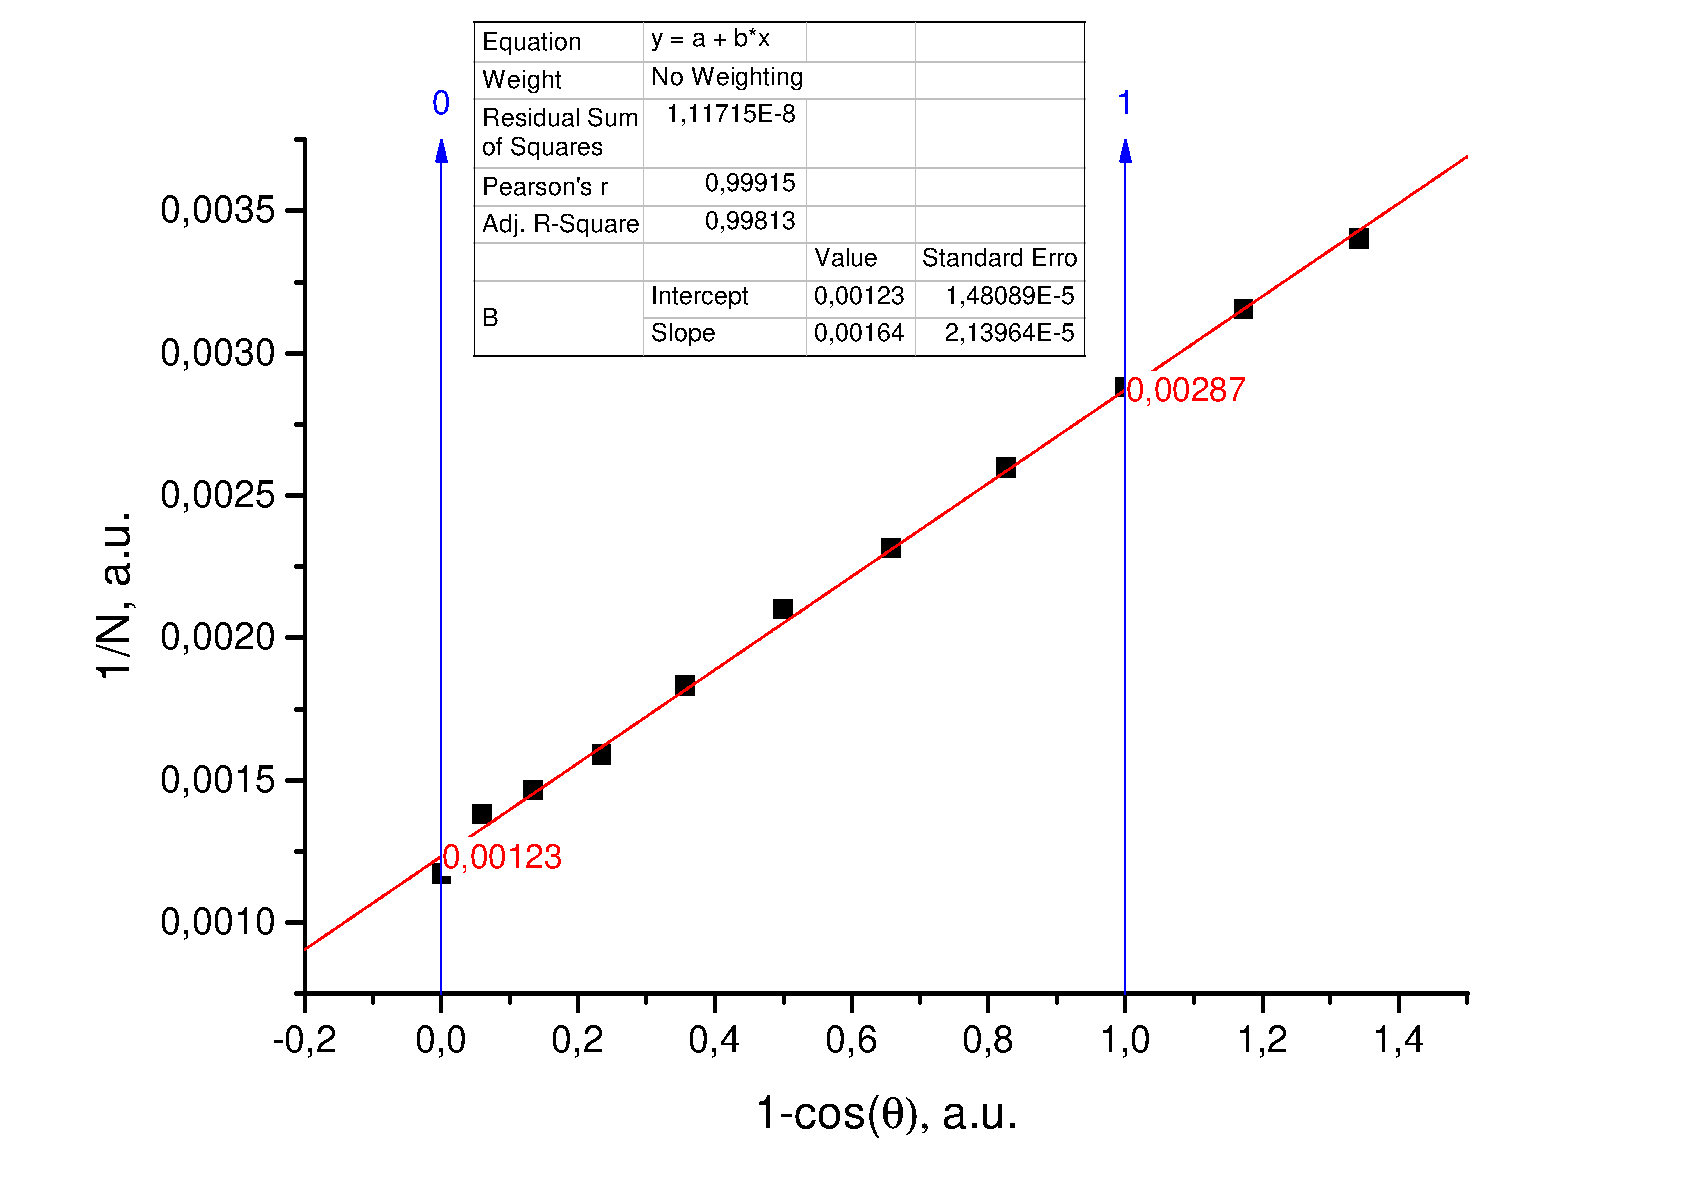
\includegraphics[width=\linewidth]{graph1}
		\end{figure}
		
		По данным графика рассчитаем энергию покоя электронов:
		\begin{equation}
			E_{r} = E_{\gamma} = \frac{N(90)}{N(0)-N(90)} = 0.662\cdot\frac{348.43}{813.01-348.43} = 0.4965\pm0.011\, \mathrm{MeV}
		\end{equation}
	\section{Обсуждение результатов и выводы}
		В ходе работы мы наблюдали рассеяние свободных гамма-квантов на свободных электронах графита. В ходе эксперимента выяснен интересный характер диаграммы направленности излучения источника $\gamma$-квантов: при больших углах обнаруживаются фоновые $\gamma$-кванты, проходящие через боковую стенку источника.  По результатам опыта была получена масса покоя электрона: $496\pm11\,\mathrm{MeV}$. Табличное значение $512\,\mathrm{MeV}$, а значит наш эксперимент находится в хорошем согласии с теорией.
					
\end{document}


